\section{Hyper-parameter Optimization}%
\label{sec:hyper_parameter_optimization}

Before a machine learning model can be trained, certain decisions regarding the
architecture of the network have to be made. This involves parameters such as
the number of layers in feedforward networks, kernel sizes in
convolutional nets or, as in the case of the ESN, sparsity and spectral radius
of the reservoir.  These parameters are called \emph{hyper-parameters} (HP) and
they fill a compact space $\mathbf{X}$.  The goal of HP optimization is to find
a configuration $\mathbf{x_i}$ that maximizes the performance of the network:
\begin{equation}
  \arg \max_{\mathbf{x_i} \in \mathbf{X}} f(\mathbf{x_i})
\end{equation}
The function $f$ is not known and very expensive to evaluate as one evaluation
amounts to the creation of a trained NN.  Often this optimization problem is
solved by handily tuning each HP until a \emph{reasonably} good
$\mathbf{x_{\text{opt}}}$ is found, but there are a few methods that can be
applied to automate this process.  The two simplest methods are \emph{grid
searches} and \emph{random searches} of the HP space.  First, the space of
valid HPs is defined.  For example, a number of units $N = (10, 20, 30,...,
100)$ and a learning rate $\eta = (0.1, 0.01, 0.001, ...)$. Grid search then
performs an exhaustive search of all parameters, which is very simple to
implement but suffers from the curse of dimensionality.  Random search randomly
samples $\mathbf{x_i}$ from the HP space, which does not have the problem of
needing to perform an exhaustive search and is widely applied in practice, as
it is still very simple to implement.

The next section describes an algorithm called \emph{Bayesian Optimization},
which also samples the next $\mathbf{x_i}$ but incorporates the knowledge of
already evaluated points in the HP space.  It utilizes Bayes' Theorem which,
adjusted to this problem, states that the \emph{posterior} probability
distribution of a model $M$ (over the HP space $\mathbf{X}$) given a number of
already evaluated samples $A \in \mathbf{X}$ is:
\begin{equation}
  P(M|A) \propto P(A|M) P(M),
\end{equation}
where $P(M)$ is the \emph{prior} probability distribution over $X$, and
$P(A|M)$ the \emph{likelihood} of the samples given $M$.


\subsection{Bayesian Optimization}%

The following description is largely based on article~[\cite{brochu2010bayesopt}]
and will briefly introduce the concept of Gaussian
Processes and how they are used in Bayesian Optimization as introduced
by~[\cite{williams1996gaussian}].  In summary, the Bayesian Optimization
algorithm tries to maximize an objective function $f$ by balancing exploration
(evaluating areas where the true values of $f$ are very uncertain) and
exploitation (which tries to evaluate $f$ where it is expected to be high). It
rests upon the concept of Gaussian Processes (GP), which can be used to define
a distribution over $f$.  From the GP it is possible to calculate an
acquisition function, which is used to efficiently sample the next
$\mathbf{x}_i$ that should be evaluated.  There are different acquisition
functions that emphasize either exploration or exploitation. The method of
Bayesian Optimization yields good results with only few evaluations and is very
likely to perform well on objective functions with local maxima.\\

\subsubsection{Gaussian Processes}%
\label{ssub:gaussian_processes}

A GP is defined by its mean function $m(\mathbf{x}_i)$ and its covariance
function $k(\mathbf{x}_i, \mathbf{x}_j)$.  This means that to each argument
$\mathbf{x}_i$ we assign a random variable $f(\mathbf{x}_i)$.  In analogy to
the Normal distribution, a GP is formally written as:
\begin{equation}
  f \sim {GP}(m,k)
\end{equation}
where $m(\mathbf{x}_i)$ can be any function but typically is just zero, and a
common covariance matrix is created with a Gaussian kernel:
\begin{equation} \label{eq:cov}
  \mathbf{K}_{ij} = k(\mathbf{x}_i, \mathbf{x}_j) =
      \exp \bigg(\frac{- ||\mathbf{x}_i - \mathbf{x}_j||^2}{2}\bigg).
\end{equation}
This kernel is close to one for values close to each other and approaches zero
as the values grow further apart, which implies that close values are highly
correlated.
With this definition, a GP is equivalent to a multivariate Gaussian
$\mathcal{N}(\mu, \Sigma)$ with mean vector $\mu$ and a covariance matrix
$\Sigma$:
\begin{align}
  \mu_i &= m(\mathbf{x}_i) \\
  \Sigma_{ij} &= k(\mathbf{x}_i, \mathbf{x}_j)
\end{align}

Given mean and covariance we can use the GP as a prior for the function $f$ of
which we want to find the maximum. By choosing a zero mean, the only actual
prior information is a smoothly operating $f$, implied by the Gaussian kernel.
The interesting part is how to update this prior with information that is
gained by evaluating $f$ a certain point to obtain a posterior.  Assuming that
we already have $n$ observations $\{\mathbf{x}_{1:n} ; f(\mathbf{x}_{1:n})\}$
we can find the covariance matrix $\mathbf{K}$ with Eq.~\ref{eq:cov}.  To find
the probability distribution of an unobserved point $\mathbf{x}_{n+1}$, the
conditional probability of $f_{n+1}$ given the previous observations (also
called predictive distribution) is needed:
\begin{equation}
  P(f_{n+1} | \mathbf{x}_{1:n} ; f(\mathbf{x}_{1:n})) 
    = \mathcal{N}(\mu_p(\mathbf{x}_{n+1}) , \sigma_p^2(\mathbf{x}_{n+1})),
\end{equation}

where $\mu_p$ and $\sigma_p$ are the predicted mean and standard deviation at
an unknown point.  They can be calculated thanks to the properties of the GP,
which state that the observations and the arbitrary point $\mathbf{x}_{n+1}$
are jointly Gaussian:
\begin{align}
  &\begin{bmatrix} f(\mathbf{x}_{1:n}) \\ f(\mathbf{x}_{n+1}) \end{bmatrix}
  \sim \mathcal{N} \bigg(
    0,  \begin{bmatrix} 
           \mathbf{K} & \mathbf{k}^T \\ 
           \mathbf{k} & k(\mathbf{x}_{n+1}, \mathbf{x}_{n+1})
        \end{bmatrix}
  \bigg) \\
  &\mathbf{k} = \begin{bmatrix}
      k(\mathbf{x}_1, \mathbf{x}_{n+1}) &
      \dots &
      k(\mathbf{x}_n, \mathbf{x}_{n+1})
  \end{bmatrix}
\end{align}

From this it is possible to derive that:
\begin{align}
  \mu_p (\mathbf{x}_{n+1}) &= \mathbf{k}^T \mathbf{K}^{-1} f(\mathbf{x}_{1:n}) \\
  \sigma_p (\mathbf{x}_{n+1}) &= k(\mathbf{x}_{n+1}, \mathbf{x}_{n+1}) 
                               - \mathbf{k}^T \mathbf{K}^{-1} \mathbf{k}
\end{align}

The resulting predictive distribution is typically very cheap to evaluate as
the number of observations is low. With this distribution it is possible
to find the so called \emph{acquisition function}, which enables an educated
guess of the next best point of evaluation of the objective function.

\label{sub:bayesian_optimization}
\begin{figure}
  \centering
  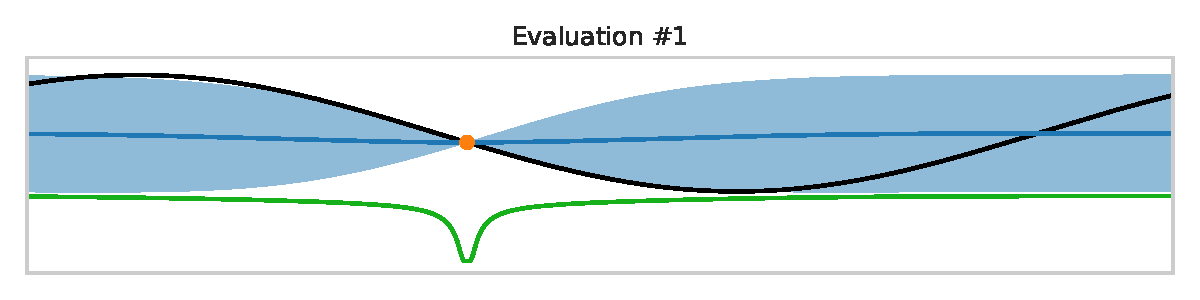
\includegraphics[width=\linewidth]{gpopt_01.pdf}
  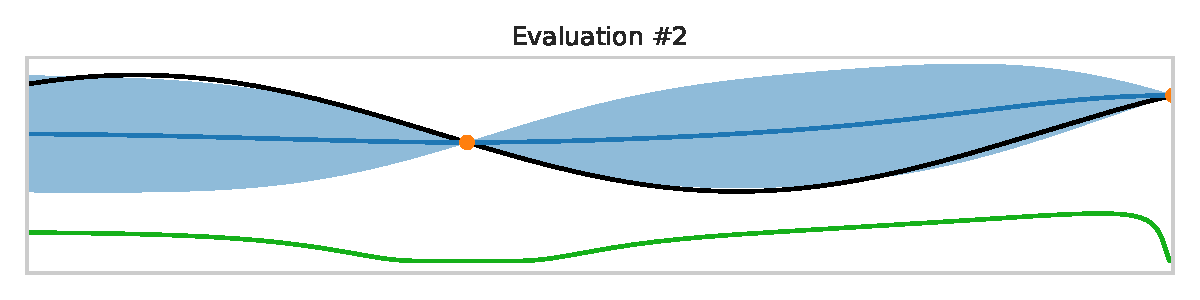
\includegraphics[width=\linewidth]{gpopt_02.pdf}
  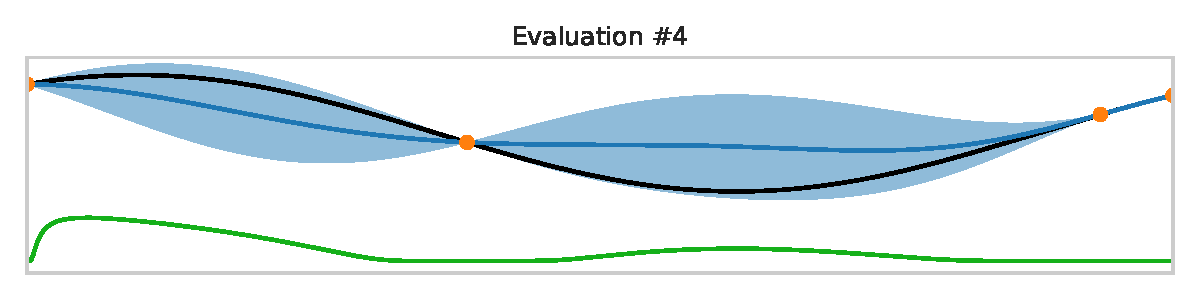
\includegraphics[width=\linewidth]{gpopt_04.pdf}
  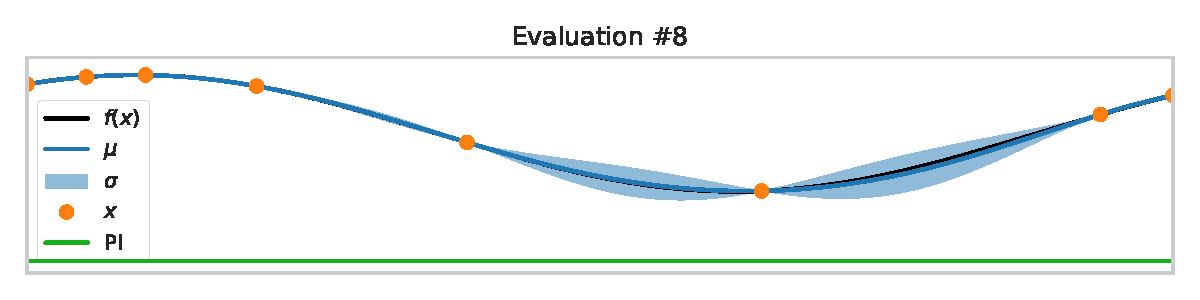
\includegraphics[width=\linewidth]{gpopt_08.pdf}
  \caption{A timeline of Bayesian Optimization. The plots show how the GP
    approximates the objective function better and better after each iteration.
    The maximum of the green acquisition function indicates where $f$ will be
    sampled next.  The uncertainty of already observed points is zero in this
    case, as there is no noise incorporated in the example. However, noisy
    objective functions can be dealt with by only slight additions to the
    described algorithm. An in depth description of Gaussian Processes and
    how they can be applied to ML can be found in~[\cite{rasmussen2004gaussian}].
  }
  \label{fig:gpopt_01}
\end{figure}


\subsubsection{Acquisition function}%
\label{ssub:acquisition_function}

The acquisition function is obtained from the predictive distribution of the 
GP and is defined such that it is high where the objective function $f$ is
\emph{potentially} high.  The probability of large objective values is high
where either the uncertainty or the mean (or both) of the GP are large. 
Maximizing the acquisition function amounts to sampling $f$ at
\begin{equation}
  \mathbf{x}_{n+1} = \arg \max_{\mathbf{x_i} \in \mathbf{X}} 
                     \text{ PI}(\mathbf{x}_i).
\end{equation}
The function PI is an example of an acquisition function called the
\emph{probability of improvement}:
\begin{align}
  \text{PI}(\mathbf{x}_i) &= P(f(\mathbf{x}_i) > f(\mathbf{x}^+)) \\
  &= \Phi\bigg( \frac{\mu_p(\mathbf{x}_i) - \mu_p(\mathbf{x}^+)}
                     {\sigma_p(\mathbf{x}_i)}  \bigg) \nonumber
\end{align}
Here $\Phi$ is the cumulative distribution function. The emphasis of PI clearly
lies on exploitation, as samples with a mean lower than the current maximal
mean will never reach PI values over 0.5.  More sophisticated acquisition
functions than PI, which are not purely driven by exploitation include
\emph{expected improvement}. A description of various acquisition functions
and Bayesian Optimization as a whole can be found in~[\cite{brochu2010bayesopt}].
